\documentclass{beamer}
\usetheme[pageofpages=of,% String used between the current page and the
                         % total page count.
          bullet=circle,% Use circles instead of squares for bullets.
          titleline=true,% Show a line below the frame title.
          alternativetitlepage=true,% Use the fancy title page.
	  titlepagelogo=logo-circl.pdf,% Logo for the first page.
%          watermark=watermark-polito,% Watermark used in every page.
%          watermarkheight=100px,% Height of the watermark.
%          watermarkheightmult=4,% The watermark image is 4 times bigger
                                % than watermarkheight.
          ]{Torino}

\usepackage[utf8x]{inputenc}
\usepackage{listings}
\usepackage{soul}
\usepackage{siunitx}
\usepackage{booktabs}
%\lstset{ 
%  backgroundcolor=\color{white},   % choose the background color; you must add \usepackage{color} or \usepackage{xcolor}
%  basicstyle=\footnotesize,        % the size of the fonts that are used for the code
%  breakatwhitespace=false
%}

\usepackage{tikz}
\usetikzlibrary{shapes,snakes,automata,positioning,matrix,fit,arrows,shapes.geometric}


\usepackage[listings]{tcolorbox}
\usepackage{xcolor}
\usepackage{colortbl}
\definecolor{mygreen}{rgb}{0,0.6,0}
\definecolor{mygreen2}{rgb}{0,0.56,0.16}
\definecolor{myred}{rgb}{0.6,0.066,0.066}
\definecolor{redCIRCL}{RGB}{213,43,30}
\definecolor{mygray}{rgb}{0.5,0.5,0.5}
\definecolor{mymauve}{rgb}{0.58,0,0.82}
\definecolor{mygray}{gray}{0.9}
\definecolor{mywhite}{rgb}{1,1,1}
\definecolor{myblack}{rgb}{0,0,0}
\definecolor{mybeige}{HTML}{eeeeee}
%\usepackage{tcolorbox}
\usepackage[listings]{tcolorbox}
\tcbuselibrary{listings}

\lstdefinestyle{code}{ %
  backgroundcolor=\color{mybeige},   % choose the background color; you must add \usepackage{color} or \usepackage{xcolor}; should come as last argument
  basicstyle=\footnotesize\ttfamily,        % the size of the fonts that are used for the code
  breakatwhitespace=false,         % sets if automatic breaks should only happen at whitespace
  breaklines=true,                 % sets automatic line breaking
  captionpos=b,                    % sets the caption-position to bottom
  commentstyle=\color{mygreen},    % comment style
  deletekeywords={...},            % if you want to delete keywords from the given language
  escapeinside={\%*}{*)},          % if you want to add LaTeX within your code
  extendedchars=true,              % lets you use non-ASCII characters; for 8-bits encodings only, does not work with UTF-8
  frame=single,	                   % adds a frame around the code
  keepspaces=true,                 % keeps spaces in text, useful for keeping indentation of code (possibly needs columns=flexible)
  keywordstyle=\color{blue},       % keyword style
  language=Python,                 % the language of the code
  morekeywords={*,...},           % if you want to add more keywords to the set
  numbers=left,                    % where to put the line-numbers; possible values are (none, left, right)
  numbersep=5pt,                   % how far the line-numbers are from the code
  numberstyle=\tiny\color{myblack}, % the style that is used for the line-numbers
  rulecolor=\color{black},         % if not set, the frame-color may be changed on line-breaks within not-black text (e.g. comments (green here))
  showspaces=false,                % show spaces everywhere adding particular underscores; it overrides 'showstringspaces'
  showstringspaces=false,          % underline spaces within strings only
  showtabs=false,                  % show tabs within strings adding particular underscores
  stepnumber=1,                    % the step between two line-numbers. If it's 1, each line will be numbered
  stringstyle=\color{mymauve},     % string literal style
  tabsize=2,	                   % sets default tabsize to 2 spaces
  title=\lstname                   % show the filename of files included with \lstinputlisting; also try caption instead of title
}
\lstdefinestyle{bash}{ %
  backgroundcolor=\color{black!85},   % choose the background color; you must add \usepackage{color} or \usepackage{xcolor}; should come as last argument
  basicstyle=\footnotesize\color{mywhite},        % the size of the fonts that are used for the code
  breakatwhitespace=false,         % sets if automatic breaks should only happen at whitespace
  breaklines=true,                 % sets automatic line breaking
  captionpos=b,                    % sets the caption-position to bottom
  commentstyle=\color{mygreen},    % comment style
  deletekeywords={...},            % if you want to delete keywords from the given language
  escapeinside={\%*}{*)},          % if you want to add LaTeX within your code
  extendedchars=true,              % lets you use non-ASCII characters; for 8-bits encodings only, does not work with UTF-8
  frame=single	                   % adds a frame around the code
  keepspaces=true,                 % keeps spaces in text, useful for keeping indentation of code (possibly needs columns=flexible)
  keywordstyle=\color{white}\bfseries,       % keyword style
  language=bash,                 % the language of the code
  morekeywords={*,$,git, clone,... },           % if you want to add more keywords to the set
  numbers=left,                    % where to put the line-numbers; possible values are (none, left, right)
  numbersep=5pt,                   % how far the line-numbers are from the code
  numberstyle=\tiny\color{mywhite}, % the style that is used for the line-numbers
  rulecolor=\color{black},         % if not set, the frame-color may be changed on line-breaks within not-black text (e.g. comments (green here))
  showspaces=false,                % show spaces everywhere adding particular underscores; it overrides 'showstringspaces'
  showstringspaces=false,          % underline spaces within strings only
  showtabs=false,                  % show tabs within strings adding particular underscores
  stepnumber=1,                    % the step between two line-numbers. If it's 1, each line will be numbered
  stringstyle=\color{mymauve},     % string literal style
  tabsize=2,	                   % sets default tabsize to 2 spaces
  title=\lstname                   % show the filename of files included with \lstinputlisting; also try caption instead of title
}
\lstdefinestyle{default}{ %
  backgroundcolor=\color{white},   % choose the background color; you must add \usepackage{color} or \usepackage{xcolor}; should come as last argument
  basicstyle=\footnotesize\color{black},        % the size of the fonts that are used for the code
  breakatwhitespace=false,         % sets if automatic breaks should only happen at whitespace
  breaklines=true,                 % sets automatic line breaking
  captionpos=b,                    % sets the caption-position to bottom
  commentstyle=\color{mygreen},    % comment style
  deletekeywords={...},            % if you want to delete keywords from the given language
  escapeinside={\%*}{*)},          % if you want to add LaTeX within your code
  extendedchars=true,              % lets you use non-ASCII characters; for 8-bits encodings only, does not work with UTF-8
  frame=single	                   % adds a frame around the code
  keepspaces=true,                 % keeps spaces in text, useful for keeping indentation of code (possibly needs columns=flexible)
  keywordstyle=\color{white}\bfseries,       % keyword style
  language=bash,                 % the language of the code
  morekeywords={*,$,git, clone,... },           % if you want to add more keywords to the set
  numbers=left,                    % where to put the line-numbers; possible values are (none, left, right)
  numbersep=5pt,                   % how far the line-numbers are from the code
  numberstyle=\tiny\color{black}, % the style that is used for the line-numbers
  rulecolor=\color{black},         % if not set, the frame-color may be changed on line-breaks within not-black text (e.g. comments (green here))
  showspaces=false,                % show spaces everywhere adding particular underscores; it overrides 'showstringspaces'
  showstringspaces=false,          % underline spaces within strings only
  showtabs=false,                  % show tabs within strings adding particular underscores
  stepnumber=1,                    % the step between two line-numbers. If it's 1, each line will be numbered
  stringstyle=\color{mymauve},     % string literal style
  tabsize=2,	                   % sets default tabsize to 2 spaces
  title=\lstname                   % show the filename of files included with \lstinputlisting; also try caption instead of title
}
\lstset{style=code}


\AtBeginSection[]{
	\begin{frame}[fragile]
  \vfill
  \centering
  \begin{beamercolorbox}[sep=8pt,center,shadow=true,rounded=true]{title}
      {\color{white} \usebeamerfont{title}\insertsectionhead}\par%
  \end{beamercolorbox}
  \vfill
  \end{frame}
}

\author{\large{Alexandre Dulaunoy}\\ \scriptsize{alexandre.dulaunoy@circl.lu}\\ \large{Jean-Louis Huynen}\\ \scriptsize{jean-louis.huynen@circl.lu}\\}
\title{Writing YARA rules}
\subtitle{An introduction to YARA for AIL usage}
\institute{info@circl.lu}
\date{\today}
\begin{document}


\begin{frame}[t,plain]
\titlepage
\end{frame}

\begin{frame}
\frametitle{Links}
    \begin{itemize}
        \item AIL project: \url{https://github.com/ail-project}
        \item AIL framework: \url{https://github.com/ail-project/ail-framework}
        \item Training materials: \url{https://github.com/ail-project/ail-training}
	\item YARA doc: \url{https://yara.readthedocs.io/en/stable/} 
	\item YARA download:  \url{http://virustotal.github.io/yara/}
    \end{itemize}
\end{frame}

\begin{frame}[fragile]
\frametitle{What's YARA?}
	\begin{itemize}
	\item {\it The pattern matching swiss knife for malware researchers (and everyone else)};
	\item It's an improved {\bf grep} to create pattern matching rule to search for {\bf strings}, {\bf binary patterns}, {\bf regular expressions};
	\item A YARA rule can be contextualised with metadata and tags describing a specific set of pattern matching rules.
	\item Easier definiton of conditions compared to regex.
	\end{itemize}
\end{frame}

\lstset{language=Python}
\begin{frame}[fragile]
\frametitle{A sample rule - disneyplus.yara}
	\begin{lstlisting}
	rule disney_plus : credential_leak 
{
    meta:                                        
        description = "Finding list of credentials for Disney Plus"
        leak = 1
    strings: 
        $a = "gmail.com:"
        $b = "DISNEY_PLUS"
        $c = "Disney Plus"
    condition:
        $a and ($b or $c) 
}
	\end{lstlisting}
\end{frame}


\lstset{language=sh}
\begin{frame}[fragile]
\frametitle{Calling yara from command line}
	\begin{itemize}
	\item Searching a single file
	\begin{lstlisting}
yara disneyplus.yara /home/adulau/dataset/2021/09/01/nv6RsKFm
	\end{lstlisting}
	\item Searching a directory
	\begin{lstlisting}
yara disneyplus.yara -r /home/adulau/dataset/2021/09/01/
	\end{lstlisting}
	\end{itemize}
\end{frame}

\begin{frame}
\frametitle{Regular Expressions}
    \begin{itemize}
        \item Regular Expressions (Regex) are extremely useful in extracting information from text
	    \item A regex is a sequence of characters that specifies a search pattern
        \item They can be used to match, locate extract and replace text
    \end{itemize}
\end{frame}

\begin{frame}[fragile]
\frametitle{Regular Expressions}
You can search for simple letters and specifiy repetition or existence

\begin{lstlisting}
String: `Cookie`

// `.` Any single character
$re1: /Co.kie/

// `*` Zero or more for the previous sequence
$re2: /Co*kie/

// `+` One or more for the previous sequence
$re3: /Co+kie/
\end{lstlisting}
\end{frame}

\begin{frame}[fragile]
\frametitle{Regular Expressions}
\begin{lstlisting}
// `{2,3}` Between 2 and 3
$re4: /Co{2,3}kie/

// `[a-zA-Z]` Any letter between `a` and `Z`
$re5: /Co[a-zA-Z]kie/ 
\end{lstlisting}
\end{frame}


\begin{frame}[fragile]
\frametitle{Regular Expressions}
Usecase: Email addresses
\begin{lstlisting}
$re1: /.+@.+\..+/ 
// The address `1@.` is valid


$re2: /.+@.+\.[a-zA-Z]{2,4}/ 
// We enforce a correct TLD (i.e. `.com`)

\end{lstlisting}
\end{frame}

\begin{frame}[fragile]
\frametitle{Regular Expressions}
Usecase: Email addresses
\begin{lstlisting}
$re2: /.+@[a-zA-Z0-9_.-]+\.[a-zA-Z]{2,4}/ 
// We enforce a correct domain (i.e. `gmail` or `hotmail`)

$re3: /[a-zA-Z0-9_.%+-]+@[a-zA-Z0-9_.-]+\.[a-zA-Z]{2,4}/ 
// We enforce a correct email format
// `!john@doe~@gmail.com` is not valid anymore

\end{lstlisting}

\begin{center}
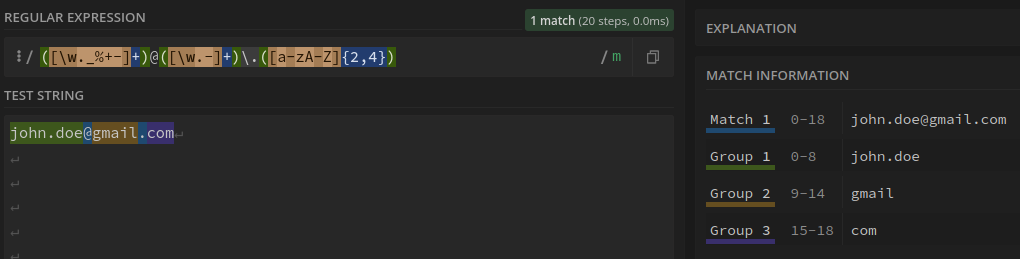
\includegraphics[width=1.0\textwidth]{pics/regex101}
\end{center}
\end{frame}


\begin{frame}[fragile]
\frametitle{Fun with Regular Expressions}
\texttt{https://regexcrossword.com/}

\begin{center}
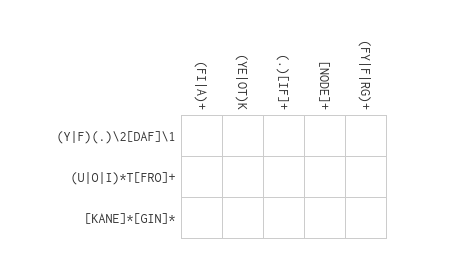
\includegraphics[width=0.8\textwidth]{pics/crosswords}
\end{center}
\end{frame}

\begin{frame}
  \frametitle{Searching in binaries}
Binaries packed with UPX but made unusable by UPX -d by modifying the magic UPX string:
  \begin{figure}[h]
    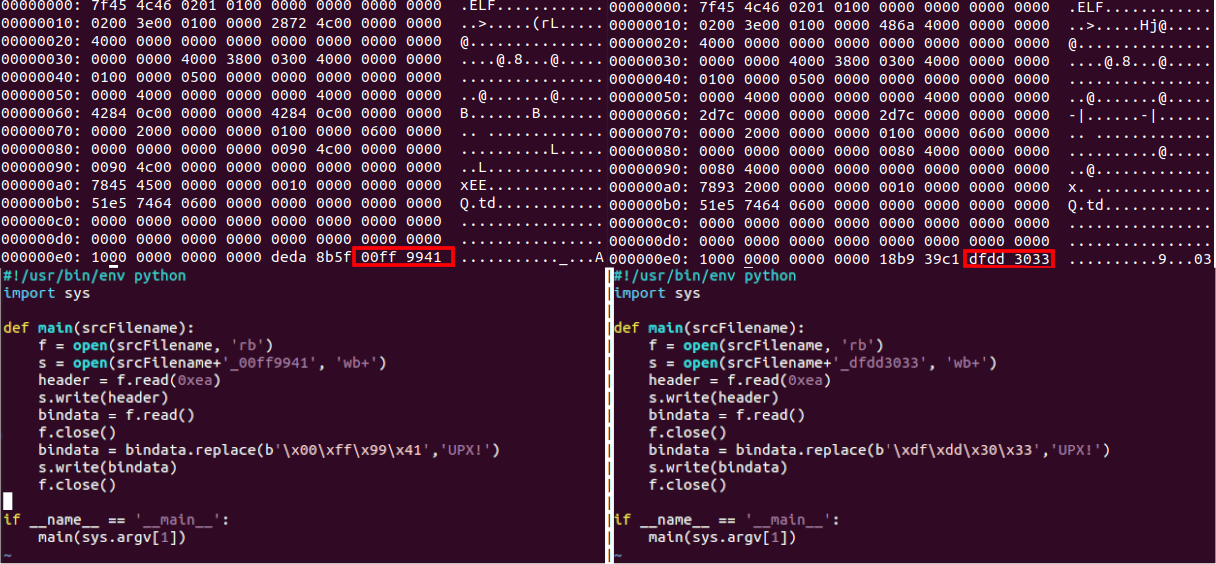
\includegraphics[width=\textwidth]{images/unpack.png}
  \end{figure}
\end{frame}

\lstset{language=Python}
\begin{frame}[fragile]
\frametitle{Searching in binaries}
	\begin{lstlisting}
rule torcryptomining
{
    strings:
        $upx_erase = {(00 FF 99 41|DF DD 30 33)}
    condition:
        $upx_erase at 236
}
	\end{lstlisting}
\end{frame}


\end{document}

